\subsection{Presentation of the interface}

	Launching the program makes the following window appear.
	\begin{figure}[H]
		\centering
		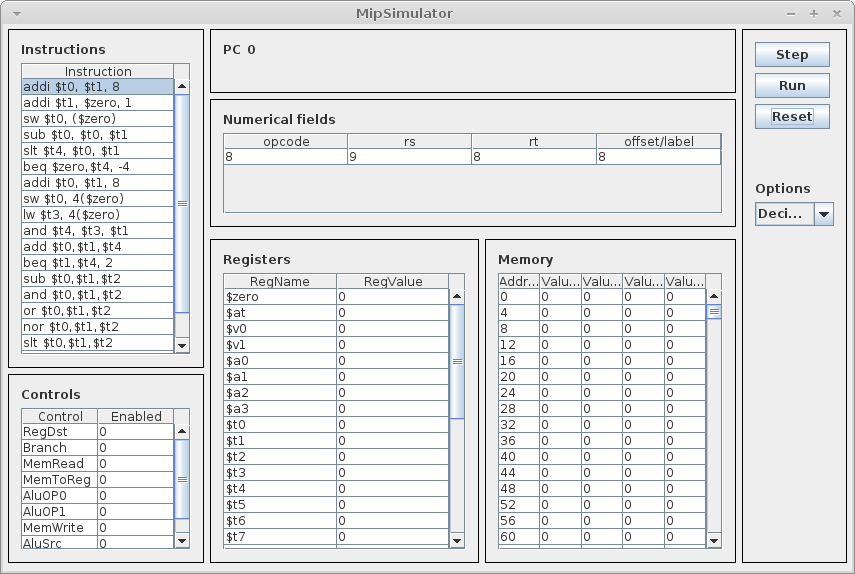
\includegraphics[scale=0.6]{img/main_window_s0.png}
		\caption{Initial state}
		\label{fig:ini_state}		
	\end{figure}
	
	By default values are displayed using decimal format. Hexadecimal format can be used and the way to switch between these two representations will be explained later.
	
	\subsubsection{Instructions frame}
	
		The instructions frame displays instructions which are in the input file using mnemonic format. The current instruction is highlighted. 

	\subsubsection{Controls frame}
	
		The controls frame displays the control lines, i.e. the boolean values used by the processor to share some command to the different units.
		
	\subsubsection{PC frame}
	
		The PC frame displays the current value of the program counter.
		
	\subsubsection{Numerical fields frame}
	
		The numerical fields frame displays values of each field of the current instruction.
		
	\subsubsection{Registers frame}
	
		The registers frame displays the value of each registers.
	
	\subsubsection{Data memory frame}
	
		The data memory frame displays the value of each memory address.
		
	\subsubsection{Step button}
	
		The step button can be used to execute the current instruction and only this one.
	
	\subsubsection{Run button}
	
		The run button can be used to execute the whole program.
		
	\subsubsection{Reset button}
	
		The reset button can be used to reset the processor and restart the program from the beginning.
		
	\subsubsection{Format switch}
	
		The format switch can be used to switch between decimal or hexadecimal representation.